\subsection{Causal isolation of the learned instruction-embedding path}
\label{app:instruction-embedding-ablation}

Token IDs are lookup addresses. A learned embedding table turns those addresses into vectors that
the policy can combine with vision and robot state. Before observing outcomes, we fixed a paired
test that isolates this conversion. On canonical episodes $30$--$39$, disjoint from the
instruction-necessity episodes, both arms received the identical correct $32$-token ID tensor. The
ablated arm replaced only the output of the token-embedding lookup with exact zeros. Sequence
length, token positions, vision, robot state, embodiment, the separate learned common BOS, action
queries, transformer weights, and action head were preserved and hash-checked.

\begin{figure}[H]
\centering
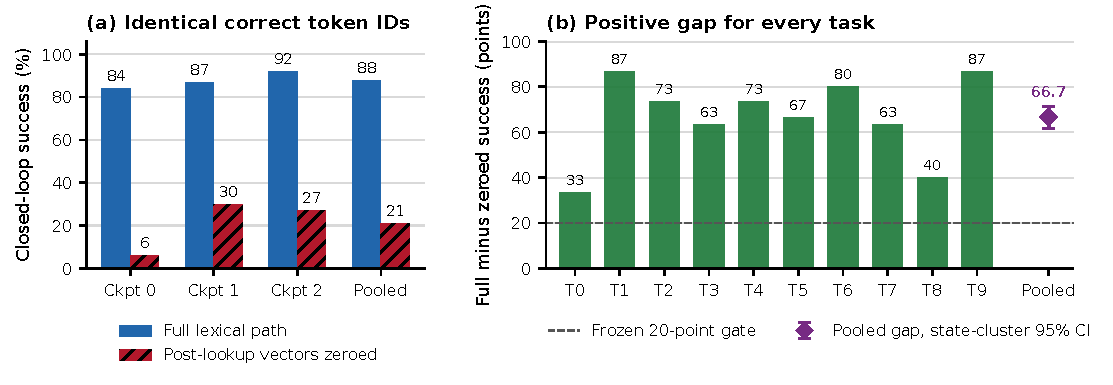
\includegraphics[width=0.98\textwidth]{../paper_figures/instruction_embedding_ablation.pdf}
\caption{\textbf{Learned lexical-embedding-path necessity on familiar tasks.} Left: closed-loop
success for the intact path and exact post-lookup zeroing, using $100$ paired states per checkpoint
and $300$ pooled pairs. Right: every task aggregate has a positive paired gap. The pooled marker
shows the frozen task-stratified state-cluster $95\%$ bootstrap interval.}
\label{fig:instruction-embedding-ablation}
\end{figure}

The intact path succeeds on $263/300=87.7\%$ of checkpoint-state pairs, compared with
$63/300=21.0\%$ after zeroing the learned token vectors. The paired gap is $66.7$ points, with
$203$ intact-only and $3$ zeroed-only outcomes. Full-path success is $84\%$, $87\%$, and $92\%$
by checkpoint, and the corresponding gaps are $78$, $57$, and $65$ points. All ten task
aggregates are positive. A pooled one-sided exact paired test gives $p=1.42\times10^{-56}$, but
this test is not cluster-robust because checkpoints reuse the same 100 states. The frozen
$20{,}000$-draw task-stratified state-cluster bootstrap interval is $[61.7,71.3]$ points and is our
cluster-aware inference. All eight prospectively fixed gates pass.

This establishes that the learned lexical-embedding path is necessary for these familiar
LIBERO-Object tasks and three fixed policies. It does not establish semantic grounding,
paraphrase robustness, unseen-object or compositional generalization, cross-suite or physical
transfer, or a benefit unique to tensor decomposability.
